%!TEX root = ../../thesis.tex

Neglecting Yukawa interactions, the EW sector of the SM contains several free 
parameters that must be experimentally determined: two couplings ($g$, $g'$) and two 
Higgs sector parameters ($\mu$, $\lambda$). Using relations in \Section~\ref{sec:ewsb}, 
it is advantageous to choose an alternative set of independent parameters more closely 
connected to experiment: \alphaEM, \mW, \mZ, \mH. Finding the Higgs boson and 
measuring its mass is therefore of fundamental importance to understanding the EW 
sector, and this was a primary goal of the LHC physics program.

Prior to the LHC, the value of \mH was constrained through direct searches at 
previous colliders, global fits of other electroweak observables and theoretical 
considerations.



\subsection{Direct searches}
\label{sec:prior_constraints:direct}

Although masses below \unit{4}{\GeV} were excluded from \PB, \PUpsilon and \PK meson 
decays \cite{PDG:1988}, the first meaningful searches for a Higgs boson were 
performed at LEP (CERN, Geneva), which ran from 1989 to 2000. This was a circular 
\epluseminus collider with a centre-of-mass (CM) energy tuned to the \PZ-pole and then 
later varied between 189 and \unit{209}{\GeV}. A combined search for \ZH was performed 
using a total integrated luminosity of \unit{2.5}{\invfb}, which excluded 
\unit{$\mH < 114.4$}{\GeV} at the 95\% confidence level (CL) \cite{LEP:2003}.

Further searches were performed at the Tevatron (FNAL, Illinois), which ran from 1987
to 2011. This was a circular \ppbar collider with CM energies of \unit{1.8}{\TeV}
and \unit{1.96}{\TeV}. In 2010, searches using a variety of production and decay modes 
were combined across experiments using a total integrated luminosity of up to
\unit{12.6}{\invfb}. Masses below \unit{109}{\GeV} and between 158 and \unit{175}{\GeV} 
were excluded at the 95\% CL \cite{Tevatron:2010}.

% \begin{figure}
% 	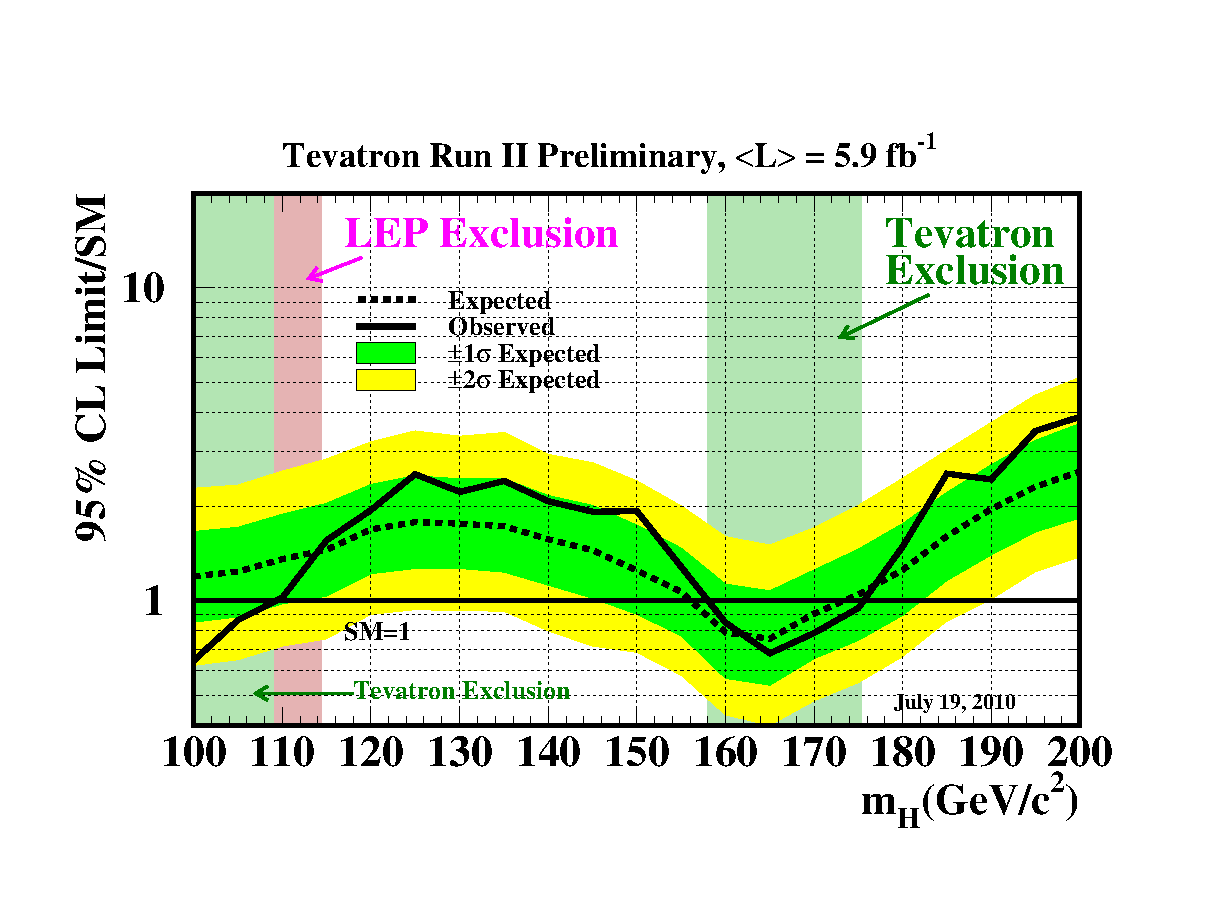
\includegraphics[width=\mediumfigwidth]{tex/motivation/tevatron_limit}
% 	\caption{Observed and expected 95\% \ac{CL} upper limits on the ratio to the \ac{SM} 
% 	cross section versus \mH, obtained through combination of multiple CDF and \dzero 
% 	analyses \cite{Tevatron:2010}. The analyses use datasets corresponding to integrated 
% 	luminosities up to \unit{5.9}{\invfb} at CDF and up to \unit{6.7}{\invfb} at \dzero.}
% 	\label{fig:existing_limits}
% \end{figure}



\subsection{Precision electroweak fits}
\label{sec:prior_constraints:ew_fits}

The SM predicts that many observables will depend upon \mH through loop corrections,
and it is therefore possible to infer \mH through precision EW measurements. Since 
the leading \mH dependence is logarithmic, the inferred constraints are weaker than those
used to predict the top mass (where the dependence is quadratic).

Performing a global fit of various electroweak measurements at the LEP, SLC and
Tevatron colliders (\eg \mW, \mZ, $m_{\Ptop}$), in July 2010 it was possible to exclude 
\mH $>$ \unit{158}{\GeV} at the 95\% CL \cite{Gfitter:2008}. However, the best fit 
value was excluded by direct searches, as shown in \Figure~\ref{fig:ewfit}.

\begin{figure}[t]
	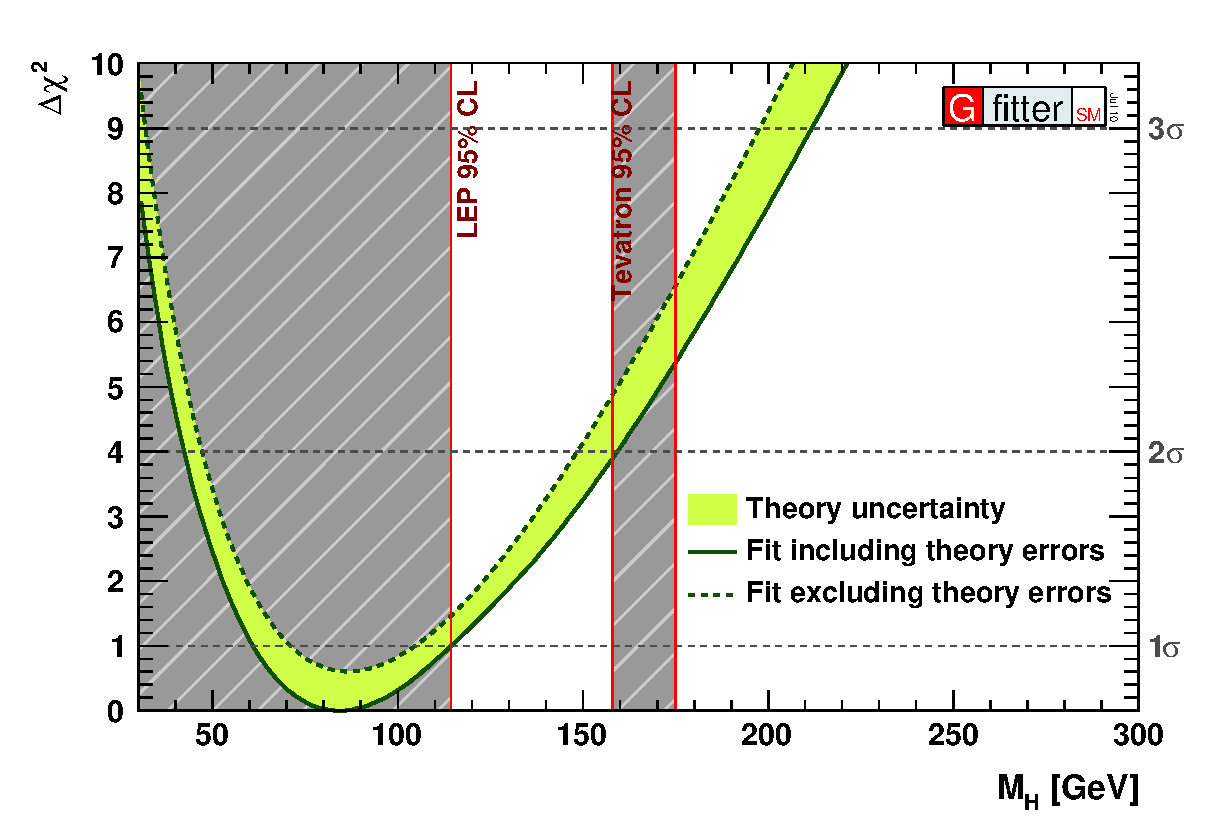
\includegraphics[width=0.495\textwidth]{tex/motivation/ewfit_nodirect}
	\hfill
	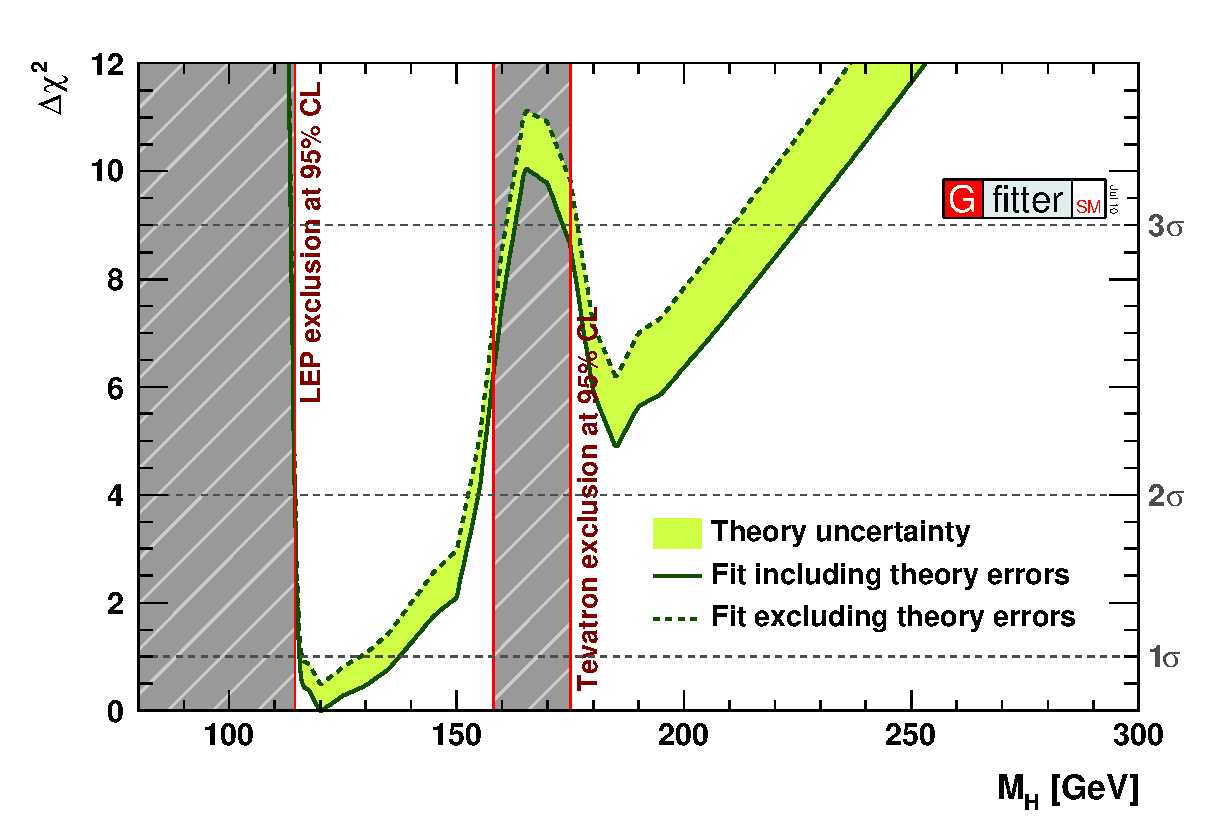
\includegraphics[width=0.495\textwidth]{tex/motivation/ewfit_withdirect}
	\caption{The observed $\Delta\chi^2 = \chi^2 - \chi^2_{\min}$ of electroweak fits 
	versus \mH, neglecting (left) and including (right) results from direct searches
	\cite{Gfitter:2008}. The exclusion limits from LEP and the Tevatron are also shown.
	These results were produced in July 2010.}
	\label{fig:ewfit}
\end{figure}

% \begin{figure}
% 	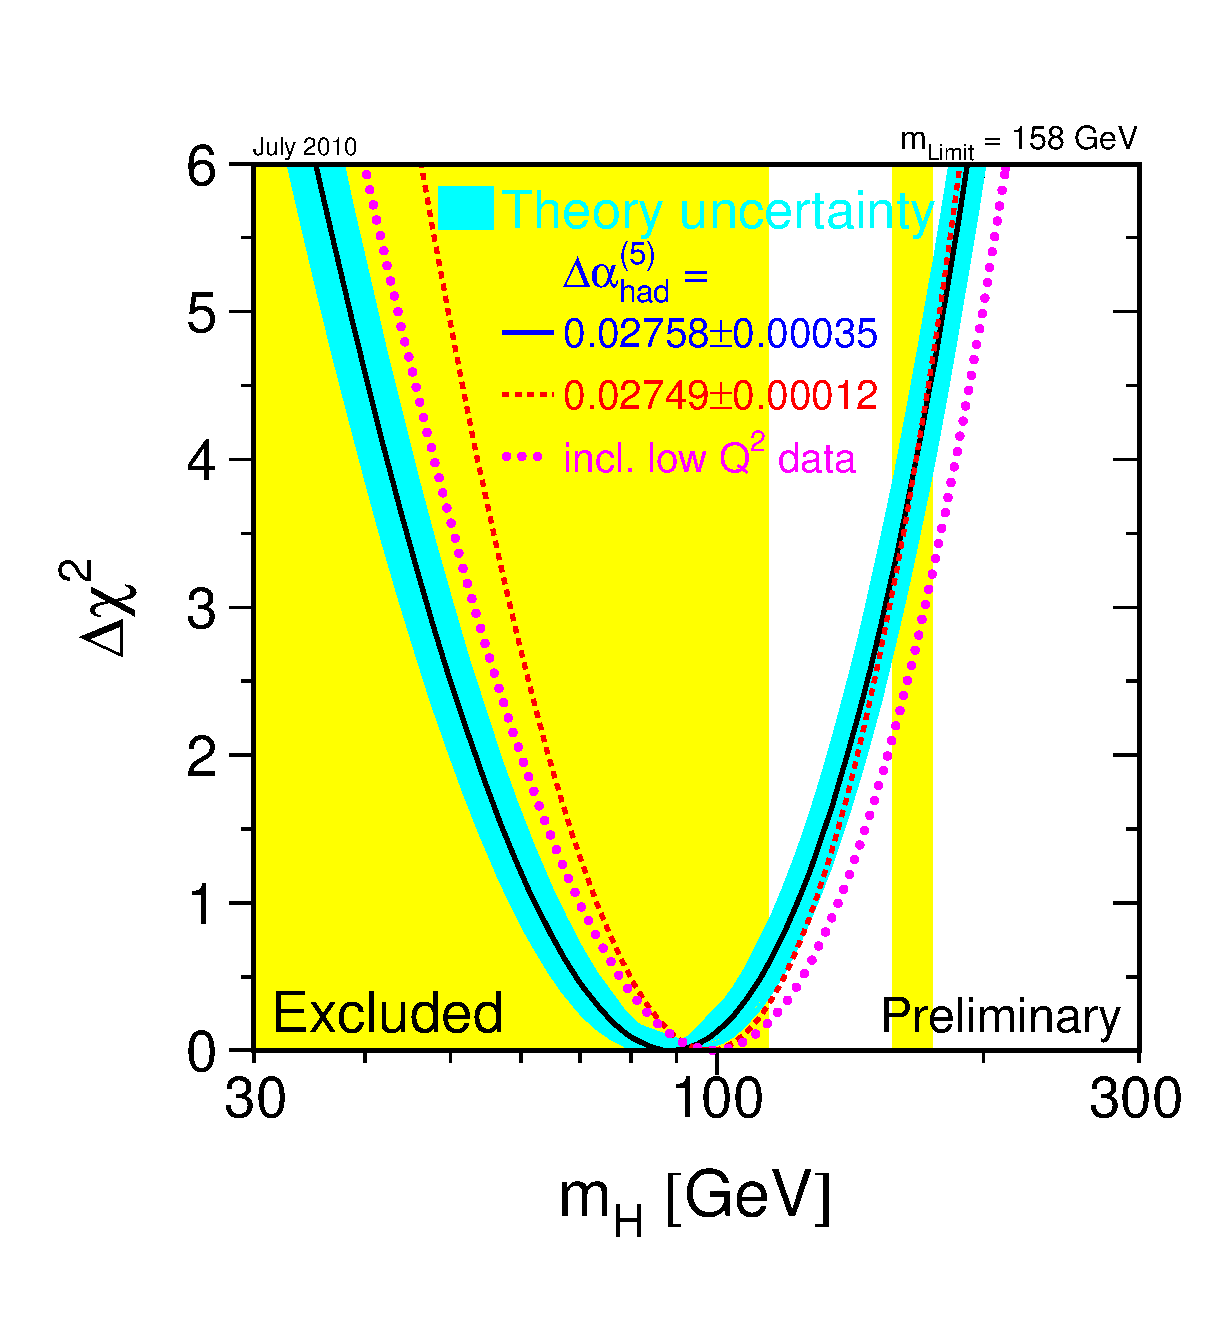
\includegraphics[width=\mediumfigwidth]{tex/motivation/ew_fit_chi2}
% 	\caption{The observed $\Delta\chi^2 = \chi^2 - \chi^2_{\min}$ of electroweak fits 
% 	versus \mH \cite{Grunewald:2010}. The line is fit using \PZ-pole data and direct 
% 	measurements of \mW, $\Gamma_{\PW}$ and $m_{\Ptop}$, and the band is an estimate of 
% 	the uncertainty due to missing higher order corrections. The dashed line uses an 
% 	alternative value of the hadronic vacuum polarisation to show the effect of 
% 	uncertainty in $\alpha(m_{\PZ}^2)$. The dotted line includes low-$Q^2$ experimental 
% 	data. The vertical bands show the 95\% \ac{CL} exclusion limits on \mH arising from 
% 	direct searches at the \ac{LEP} and the Tevatron.}
% 	\label{fig:ewfit}
% \end{figure}



\subsection{Theoretical constraints}
\label{sec:prior_constraints:theory}

Like all coupling constants in a renormalisable theory (see 
\Section~\ref{sec:qcd:renormalisation}), the Higgs quartic coupling $\lambda$ `runs' with 
energy scale $\Lambda$, as described by the renormalisation group equations (RGEs). The 
running is characterised by the $\beta$-function:
\begin{equation*}
	\beta_{\lambda} = \frac{\partial \lambda}{\partial \log\Lambda} \,.
\end{equation*}

For high \mH, self-couplings dominate $\beta_{\lambda}$, which have a
positive contribution. Therefore $\lambda$ increases with the scale, and above some 
critical scale $\Lambda_{\text{c}}$ the EW theory is no longer perturbative. Thus we 
would either expect to observe non-perturbative behaviour at scales 
\about$\Lambda_{\text{c}}$ or new physics at a scale $<\Lambda_{\text{c}}$ that 
circumvents this issue. Larger values of \mH lead to lower values of $\Lambda_{\text{c}}$ 
and are therefore disfavoured (blue line in \Figure~\ref{fig:theory_constraints}). 
Requiring perturbativity up to the reduced Planck scale of 
\unit{$\bar{\Lambda}_{\text{P}}~\about~10^{18}$}{\GeV} (where we expect new physics 
describing gravity) places an upper bound on \mH of \unit{175}{\GeV} \cite{Ellis:2009}.

For small \mH, top loops dominate $\beta_{\lambda}$, which have a negative 
contribution. Therefore $\lambda$ decreases as the scale increases, and above some 
critical scale $\Lambda_{\text{c}}$ the coupling becomes negative. Then the EW 
vacuum is simply a local minimum and it is possible for the Universe to collapse through
quantum tunnelling into the more stable vacuum state (yellow band in 
\Figure~\ref{fig:theory_constraints}). Requiring vacuum stability up to 
$\bar{\Lambda}_{\text{P}}$ places a lower bound on \mH of \unit{129}{\GeV} 
\cite{Ellis:2009}. 
It is also possible to consider a metastable Universe whose expected lifetime is longer 
than its age. Accounting for thermal fluctuations up to temperatures 
\about$\bar{\Lambda}_{\text{P}}$, the EW vacuum has a lifetime longer than the age 
of the Universe if \mH $>$ \unit{122}{\GeV} (pale blue band in 
\Figure~\ref{fig:theory_constraints}) \cite{Ellis:2009}. These bounds are rather 
sensitive to the top mass, which is 
\unit{$m_{\Ptop} = 173.18 \pm 0.94$}{\GeV} \cite{TopMass}.

\begin{figure}[t]
	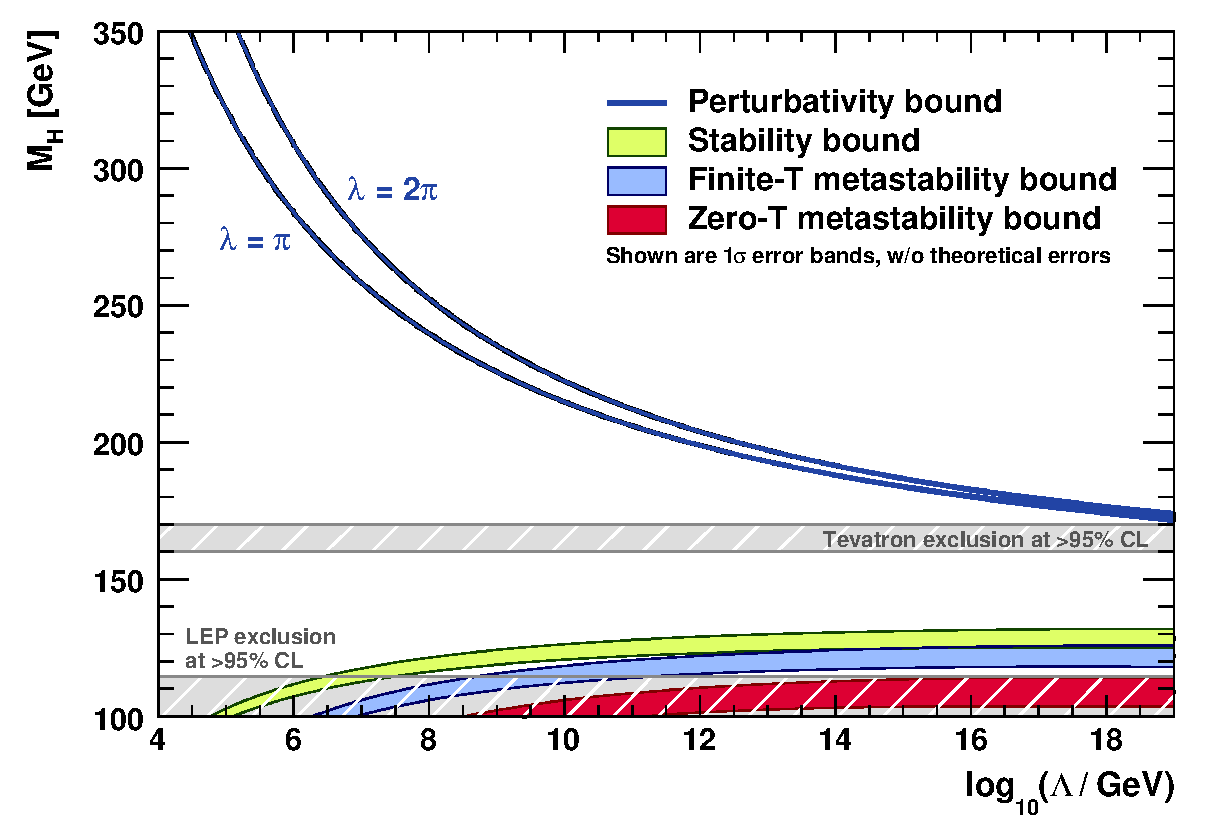
\includegraphics[width=\mediumfigwidth]{tex/motivation/theory_constraints}
	\caption{The scale $\Lambda$ at which the Higgs quartic coupling becomes 
	non-perturbative (blue lines) or an instability in the EW vacuum appears
	(yellow band) \cite{Ellis:2009}. The two blue lines represent different degrees of 
	non-perturbativity (lower line corresponds to a two-loop correction of 25\%, upper 
	line is 50\%), and their difference is indicative of the theoretical uncertainty in 
	this bound. The blue and red bands are bounds for a metastable Universe including and
	neglecting thermal fluctuations respectively.}
	\label{fig:theory_constraints}
\end{figure}
